
%% bare_conf.tex
%% V1.3
%% 2007/01/11
%% by Michael Shell
%% See:
%% http://www.michaelshell.org/
%% for current contact information.
%%
%% This is a skeleton file demonstrating the use of IEEEtran.cls
%% (requires IEEEtran.cls version 1.7 or later) with an IEEE conference paper.
%%
%% Support sites:
%% http://www.michaelshell.org/tex/ieeetran/
%% http://www.ctan.org/tex-archive/macros/latex/contrib/IEEEtran/
%% and
%% http://www.ieee.org/

%%*************************************************************************
%% Legal Notice:
%% This code is offered as-is without any warranty either expressed or
%% implied; without even the implied warranty of MERCHANTABILITY or
%% FITNESS FOR A PARTICULAR PURPOSE! 
%% User assumes all risk.
%% In no event shall IEEE or any contributor to this code be liable for
%% any damages or losses, including, but not limited to, incidental,
%% consequential, or any other damages, resulting from the use or misuse
%% of any information contained here.
%%
%% All comments are the opinions of their respective authors and are not
%% necessarily endorsed by the IEEE.
%%
%% This work is distributed under the LaTeX Project Public License (LPPL)
%% ( http://www.latex-project.org/ ) version 1.3, and may be freely used,
%% distributed and modified. A copy of the LPPL, version 1.3, is included
%% in the base LaTeX documentation of all distributions of LaTeX released
%% 2003/12/01 or later.
%% Retain all contribution notices and credits.
%% ** Modified files should be clearly indicated as such, including  **
%% ** renaming them and changing author support contact information. **
%%
%% File list of work: IEEEtran.cls, IEEEtran_HOWTO.pdf, bare_adv.tex,
%%                    bare_conf.tex, bare_jrnl.tex, bare_jrnl_compsoc.tex
%%*************************************************************************

% *** Authors should verify (and, if needed, correct) their LaTeX system  ***
% *** with the testflow diagnostic prior to trusting their LaTeX platform ***
% *** with production work. IEEE's font choices can trigger bugs that do  ***
% *** not appear when using other class files.                            ***
% The testflow support page is at:
% http://www.michaelshell.org/tex/testflow/



% Note that the a4paper option is mainly intended so that authors in
% countries using A4 can easily print to A4 and see how their papers will
% look in print - the typesetting of the document will not typically be
% affected with changes in paper size (but the bottom and side margins will).
% Use the testflow package mentioned above to verify correct handling of
% both paper sizes by the user's LaTeX system.
%
% Also note that the "draftcls" or "draftclsnofoot", not "draft", option
% should be used if it is desired that the figures are to be displayed in
% draft mode.
%
\documentclass[conference]{IEEEtran}
% Add the compsoc option for Computer Society conferences.
%
% If IEEEtran.cls has not been installed into the LaTeX system files,
% manually specify the path to it like:
% \documentclass[conference]{../sty/IEEEtran}





% Some very useful LaTeX packages include:
% (uncomment the ones you want to load)


% *** MISC UTILITY PACKAGES ***
%
%\usepackage{ifpdf}
% Heiko Oberdiek's ifpdf.sty is very useful if you need conditional
% compilation based on whether the output is pdf or dvi.
% usage:
% \ifpdf
%   % pdf code
% \else
%   % dvi code
% \fi
% The latest version of ifpdf.sty can be obtained from:
% http://www.ctan.org/tex-archive/macros/latex/contrib/oberdiek/
% Also, note that IEEEtran.cls V1.7 and later provides a builtin
% \ifCLASSINFOpdf conditional that works the same way.
% When switching from latex to pdflatex and vice-versa, the compiler may
% have to be run twice to clear warning/error messages.






% *** CITATION PACKAGES ***
%
%\usepackage{cite}
% cite.sty was written by Donald Arseneau
% V1.6 and later of IEEEtran pre-defines the format of the cite.sty package
% \cite{} output to follow that of IEEE. Loading the cite package will
% result in citation numbers being automatically sorted and properly
% "compressed/ranged". e.g., [1], [9], [2], [7], [5], [6] without using
% cite.sty will become [1], [2], [5]--[7], [9] using cite.sty. cite.sty's
% \cite will automatically add leading space, if needed. Use cite.sty's
% noadjust option (cite.sty V3.8 and later) if you want to turn this off.
% cite.sty is already installed on most LaTeX systems. Be sure and use
% version 4.0 (2003-05-27) and later if using hyperref.sty. cite.sty does
% not currently provide for hyperlinked citations.
% The latest version can be obtained at:
% http://www.ctan.org/tex-archive/macros/latex/contrib/cite/
% The documentation is contained in the cite.sty file itself.




% *** GRAPHICS RELATED PACKAGES ***
%

%\usepackage[pdftex]{graphicx}
  % declare the path(s) where your graphic files are
%\graphicspath{{images/}}
  % and their extensions so you won't have to specify these with
  % every instance of \includegraphics
  % \DeclareGraphicsExtensions{.pdf,.jpeg,.png}

  % or other class option (dvipsone, dvipdf, if not using dvips). graphicx
  % will default to the driver specified in the system graphics.cfg if no
  % driver is specified.
\usepackage[dvips]{graphicx}
  % declare the path(s) where your graphic files are
\graphicspath{{images/}}
  % and their extensions so you won't have to specify these with
  % every instance of \includegraphics
  % \DeclareGraphicsExtensions{.eps}

% graphicx was written by David Carlisle and Sebastian Rahtz. It is
% required if you want graphics, photos, etc. graphicx.sty is already
% installed on most LaTeX systems. The latest version and documentation can
% be obtained at: 
% http://www.ctan.org/tex-archive/macros/latex/required/graphics/
% Another good source of documentation is "Using Imported Graphics in
% LaTeX2e" by Keith Reckdahl which can be found as epslatex.ps or
% epslatex.pdf at: http://www.ctan.org/tex-archive/info/
%
% latex, and pdflatex in dvi mode, support graphics in encapsulated
% postscript (.eps) format. pdflatex in pdf mode supports graphics
% in .pdf, .jpeg, .png and .mps (metapost) formats. Users should ensure
% that all non-photo figures use a vector format (.eps, .pdf, .mps) and
% not a bitmapped formats (.jpeg, .png). IEEE frowns on bitmapped formats
% which can result in "jaggedy"/blurry rendering of lines and letters as
% well as large increases in file sizes.
%
% You can find documentation about the pdfTeX application at:
% http://www.tug.org/applications/pdftex





% *** MATH PACKAGES ***
%
%\usepackage[cmex10]{amsmath}
% A popular package from the American Mathematical Society that provides
% many useful and powerful commands for dealing with mathematics. If using
% it, be sure to load this package with the cmex10 option to ensure that
% only type 1 fonts will utilized at all point sizes. Without this option,
% it is possible that some math symbols, particularly those within
% footnotes, will be rendered in bitmap form which will result in a
% document that can not be IEEE Xplore compliant!
%
% Also, note that the amsmath package sets \interdisplaylinepenalty to 10000
% thus preventing page breaks from occurring within multiline equations. Use:
%\interdisplaylinepenalty=2500
% after loading amsmath to restore such page breaks as IEEEtran.cls normally
% does. amsmath.sty is already installed on most LaTeX systems. The latest
% version and documentation can be obtained at:
% http://www.ctan.org/tex-archive/macros/latex/required/amslatex/math/





% *** SPECIALIZED LIST PACKAGES ***
%
\usepackage{algorithmicx}
% algorithmic.sty was written by Peter Williams and Rogerio Brito.
% This package provides an algorithmic environment fo describing algorithms.
% You can use the algorithmic environment in-text or within a figure
% environment to provide for a floating algorithm. 
%Do NOT use the algorithm
% floating environment provided by algorithm.sty (by the same authors) or
% algorithm2e.sty (by Christophe Fiorio) as IEEE does not use dedicated
% algorithm float types and packages that provide these will not provide
% correct IEEE style captions. 
%The latest version and documentation of algorithmic.sty can be obtained at:
% http://www.ctan.org/tex-archive/macros/latex/contrib/algorithms/
% There is also a support site at:
% http://algorithms.berlios.de/index.html
% Also of interest may be the (relatively newer and more customizable)
% algorithmicx.sty package by Szasz Janos:
% http://www.ctan.org/tex-archive/macros/latex/contrib/algorithmicx/




% *** ALIGNMENT PACKAGES ***
%
%\usepackage{array}
% Frank Mittelbach's and David Carlisle's array.sty patches and improves
% the standard LaTeX2e array and tabular environments to provide better
% appearance and additional user controls. As the default LaTeX2e table
% generation code is lacking to the point of almost being broken with
% respect to the quality of the end results, all users are strongly
% advised to use an enhanced (at the very least that provided by array.sty)
% set of table tools. array.sty is already installed on most systems. The
% latest version and documentation can be obtained at:
% http://www.ctan.org/tex-archive/macros/latex/required/tools/


%\usepackage{mdwmath}
%\usepackage{mdwtab}
% Also highly recommended is Mark Wooding's extremely powerful MDW tools,
% especially mdwmath.sty and mdwtab.sty which are used to format equations
% and tables, respectively. The MDWtools set is already installed on most
% LaTeX systems. The lastest version and documentation is available at:
% http://www.ctan.org/tex-archive/macros/latex/contrib/mdwtools/


% IEEEtran contains the IEEEeqnarray family of commands that can be used to
% generate multiline equations as well as matrices, tables, etc., of high
% quality.


%\usepackage{eqparbox}
% Also of notable interest is Scott Pakin's eqparbox package for creating
% (automatically sized) equal width boxes - aka "natural width parboxes".
% Available at:
% http://www.ctan.org/tex-archive/macros/latex/contrib/eqparbox/





% *** SUBFIGURE PACKAGES ***
%\usepackage[tight,footnotesize]{subfigure}
% subfigure.sty was written by Steven Douglas Cochran. This package makes it
% easy to put subfigures in your figures. e.g., "Figure 1a and 1b". For IEEE
% work, it is a good idea to load it with the tight package option to reduce
% the amount of white space around the subfigures. subfigure.sty is already
% installed on most LaTeX systems. The latest version and documentation can
% be obtained at:
% http://www.ctan.org/tex-archive/obsolete/macros/latex/contrib/subfigure/
% subfigure.sty has been superceeded by subfig.sty.



%\usepackage[caption=false]{caption}
%\usepackage[font=footnotesize]{subfig}
% subfig.sty, also written by Steven Douglas Cochran, is the modern
% replacement for subfigure.sty. However, subfig.sty requires and
% automatically loads Axel Sommerfeldt's caption.sty which will override
% IEEEtran.cls handling of captions and this will result in nonIEEE style
% figure/table captions. To prevent this problem, be sure and preload
% caption.sty with its "caption=false" package option. This is will preserve
% IEEEtran.cls handing of captions. Version 1.3 (2005/06/28) and later 
% (recommended due to many improvements over 1.2) of subfig.sty supports
% the caption=false option directly:
%\usepackage[caption=false,font=footnotesize]{subfig}
%
% The latest version and documentation can be obtained at:
% http://www.ctan.org/tex-archive/macros/latex/contrib/subfig/
% The latest version and documentation of caption.sty can be obtained at:
% http://www.ctan.org/tex-archive/macros/latex/contrib/caption/




% *** FLOAT PACKAGES ***
%
%\usepackage{fixltx2e}
% fixltx2e, the successor to the earlier fix2col.sty, was written by
% Frank Mittelbach and David Carlisle. This package corrects a few problems
% in the LaTeX2e kernel, the most notable of which is that in current
% LaTeX2e releases, the ordering of single and double column floats is not
% guaranteed to be preserved. Thus, an unpatched LaTeX2e can allow a
% single column figure to be placed prior to an earlier double column
% figure. The latest version and documentation can be found at:
% http://www.ctan.org/tex-archive/macros/latex/base/



%\usepackage{stfloats}
% stfloats.sty was written by Sigitas Tolusis. This package gives LaTeX2e
% the ability to do double column floats at the bottom of the page as well
% as the top. (e.g., "\begin{figure*}[!b]" is not normally possible in
% LaTeX2e). It also provides a command:
%\fnbelowfloat
% to enable the placement of footnotes below bottom floats (the standard
% LaTeX2e kernel puts them above bottom floats). This is an invasive package
% which rewrites many portions of the LaTeX2e float routines. It may not work
% with other packages that modify the LaTeX2e float routines. The latest
% version and documentation can be obtained at:
% http://www.ctan.org/tex-archive/macros/latex/contrib/sttools/
% Documentation is contained in the stfloats.sty comments as well as in the
% presfull.pdf file. Do not use the stfloats baselinefloat ability as IEEE
% does not allow \baselineskip to stretch. Authors submitting work to the
% IEEE should note that IEEE rarely uses double column equations and
% that authors should try to avoid such use. Do not be tempted to use the
% cuted.sty or midfloat.sty packages (also by Sigitas Tolusis) as IEEE does
% not format its papers in such ways.





% *** PDF, URL AND HYPERLINK PACKAGES ***
%
%\usepackage{url}
% url.sty was written by Donald Arseneau. It provides better support for
% handling and breaking URLs. url.sty is already installed on most LaTeX
% systems. The latest version can be obtained at:
% http://www.ctan.org/tex-archive/macros/latex/contrib/misc/
% Read the url.sty source comments for usage information. Basically,
% \url{my_url_here}.





% *** Do not adjust lengths that control margins, column widths, etc. ***
% *** Do not use packages that alter fonts (such as pslatex).         ***
% There should be no need to do such things with IEEEtran.cls V1.6 and later.
% (Unless specifically asked to do so by the journal or conference you plan
% to submit to, of course. )


% correct bad hyphenation here
\hyphenation{op-tical net-works semi-conduc-tor}


\begin{document}
%
% paper title
% can use linebreaks \\ within to get better formatting as desired
\title{Society News Detection System}


% author names and affiliations
% use a multiple column layout for up to three different
% affiliations
\author{\IEEEauthorblockN{Chen Jie}
\IEEEauthorblockA{School of Computer Science\\
Beijing Institute of technology\\
Beijing, Haidian district\\
Email: sonyfe25cp@gmail.com}
\and
\IEEEauthorblockN{Zhendong Niu}
\IEEEauthorblockA{School of Computer Science\\
Beijing Institute of technology\\
Beijing, Haidian district\\
zniu@bit.edu.cn}
\and
\IEEEauthorblockN{Yulong Shi\\ and Changmin Zhang}
\IEEEauthorblockA{School of Computer Science\\
Beijing Institute of technology\\
Beijing, Haidian district\\
}
}

% conference papers do not typically use \thanks and this command
% is locked out in conference mode. If really needed, such as for
% the acknowledgment of grants, issue a \IEEEoverridecommandlockouts
% after \documentclass

% for over three affiliations, or if they all won't fit within the width
% of the page, use this alternative format:
% 
%\author{\IEEEauthorblockN{Michael Shell\IEEEauthorrefmark{1},
%Homer Simpson\IEEEauthorrefmark{2},
%James Kirk\IEEEauthorrefmark{3}, 
%Montgomery Scott\IEEEauthorrefmark{3} and
%Eldon Tyrell\IEEEauthorrefmark{4}}
%\IEEEauthorblockA{\IEEEauthorrefmark{1}School of Electrical and Computer Engineering\\
%Georgia Institute of Technology,
%Atlanta, Georgia 30332--0250\\ Email: see http://www.michaelshell.org/contact.html}
%\IEEEauthorblockA{\IEEEauthorrefmark{2}Twentieth Century Fox, Springfield, USA\\
%Email: homer@thesimpsons.com}
%\IEEEauthorblockA{\IEEEauthorrefmark{3}Starfleet Academy, San Francisco, California 96678-2391\\
%Telephone: (800) 555--1212, Fax: (888) 555--1212}
%\IEEEauthorblockA{\IEEEauthorrefmark{4}Tyrell Inc., 123 Replicant Street, Los Angeles, California 90210--4321}}

% use for special paper notices
%\IEEEspecialpapernotice{(Invited Paper)}

% make the title area
\maketitle


\begin{abstract}
%\boldmath
Since so many news media ouput huge volume web news, it's hard for people to know how many events happened everyday and how is the progress of some event . In this paper, we report a society news event detection system ,which help people to get the lastest event occured. The system contains three parts: society news qcquisition module , event detection module and event summariation module.
\end{abstract}
% IEEEtran.cls defaults to using nonbold math in the Abstract.
% This preserves the distinction between vectors and scalars. However,
% if the conference you are submitting to favors bold math in the abstract,
% then you can use LaTeX's standard command \boldmath at the very start
% of the abstract to achieve this. Many IEEE journals/conferences frown on
% math in the abstract anyway.

% no keywords




% For peer review papers, you can put extra information on the cover
% page as needed:
% \ifCLASSOPTIONpeerreview
% \begin{center} \bfseries EDICS Category: 3-BBND \end{center}
% \fi
%
% For peerreview papers, this IEEEtran command inserts a page break and
% creates the second title. It will be ignored for other modes.
\IEEEpeerreviewmaketitle

\section{Introduction}
% no \IEEEPARstart
With the rapid progress of technologies for information dissemination, more and more people choose Internet media instead of traditional ones as their main way to get fresh information. As a result, online news platform, one of the most important network information forms, gets a rapid growth during the past few years. Most of the popular websites have their own online news platform to attract more visitors since it is fast and real-time to get the latest trends. However, preciously because of the rapid expansion of online news, it is more and more difficult to find out valuable information from such large scale data. Especially when we want to know the development of some special events quickly, we must spend time searching and filtering out noises to get what we want by ourselves which leads a bad user experience. Event detection system which can gather relevant news and reports describing the same event automatically comes into being in such a case.

Event is a series of activities occurring at specific time and specific place, involving specific subjects and along with some consequences. It normally consists of news and reports with the same topic and has the following features. Firstly, all of these news and reports have a same topic, namely, they all describe a same event. Secondly, these reports reflect the development and latest trends of an event. For example, reports about the eruption of earthquake in Yaan and the following series of news about casualties and rescues all belong to the same event. Thirdly, all relevant reports should be included in the event.

In this paper, we design an event detection system based on J2EE aiming at providing an efficient service to users. Our system can extract news from popular news websites, aggregate all the relevant news describing the same event together automatically and display them in event forms. It is easy for users to scan and get a global picture about an event which is time saving and has a very high practical value. And also, our system can detect the newest report about the current event and add it to the news set in near real time which is a new feature of our system compared to those old ones.

The remainder of this paper is organized as follows: Section 2 reviews some related works on event detecting system. We discuss the framework, functions and some techniques used in our system in Section 3. Our experiments and the analysis of the results are described in Section 4. Section 5 presents our future plans.

% You must have at least 2 lines in the paragraph with the drop letter
% (should never be an issue)
%I wish you the best of success.

\section{Related works}

Event discovery is one practical application of the technique of topic detection and tracking. At present, most of the event detection systems are completed based on document cluster and vector space model (VSM) technologies and researchers have came up with a series of algorithms and methodologies, such as hierarchical clustering, single-pass clustering, incremental K-medoids clustering, etc.

D.Trieschnigg\cite{2005-Trieschnigg-p55-62} put forward a scalable hierarchical theme detection model. Unlike\cite{2007-Pons-Porrata-p752-768}, A.P.Porrata et al. came up with an improved incremental hierarchical clustering algorithm to detect topics by combining classification and hierarchical clustering technologies. Huang et al. \cite{2011-Huang-p280-284} put forward a novel news event detection method by using named entity when clustering. Yang \cite{2010-Yang-p372-374} analyzed the characteristics of social network such as microblog and BBS, and came up with an approach of detecting news event from noisy textual datasets. Besides text itself, we can also use other information to improve the detection probability when detecting events from news stream. Sun et al. \cite{2011-Sun-p834-839} suggested a query-guided news event detection method by analyzing user’s query, news’ title and content. Dai et al. \cite{2010-Dai-p3341-3346} thought that terms located at different areas have different distributions to similarity. For example, terms in title should make greater contribution than those in body. Based on the theory, Dai et al. put forward an improved hierarchical clustering algorithm to detect topics and an improved single-pass clustering method to track topics.

Discovering new event, the task of which is to decide which event we should locate a new report to, is one of the important modules of event detection technique. Papka et al.\cite{1998-Papka-p-} put forward a single-pass clustering approach. Firstly, they preprocessed a new coming news report and converted it to weighted vectors. Then, they calculated the similarities between the new coming news report and each of the existing records. Finally, they defined the new coming news to a new event if all of the similarities are less than the threshold. Lam et al. \cite{2001-Lam-p525-546} compared the similarities between the new coming report and all the detected events. Then they allocated the report to the cluster which has the largest similarity with it if the similarity is larger than the threshold. Otherwise, they defined a new event to hold the new coming report. Jia et al. \cite{2004-JIA-p32-32} put forward an algorithm based on dynamic evolution model to detect and track news event by combining single-pass clustering and news characteristics. 

In this paper, we design a news event detection system based on J2EE techniques. Firstly, we crawl news web pages from some popular websites using web crawlers and extract content from these web pages. Secondly, we calculate the similarities between these news reports. Thirdly, we use undirected graph to cluster the web pages with the same topic together to generate the corresponding events.

\section{System Architecture and Function Design}
In this chapter, we firstly introduce our system architecture and work flow briefly. And then we will discuss the key functional modules and key techniques we used in detail.
\subsection{System Framework}
Our system is based on J2EE framework and has 4 main modules: news crawling, content extracting, similarity computing and event discovering. And all the three former ones are the preparation stages of the last one. The work flow is as follows: Firstly, crawl all the news web pages from specified websites using web crawlers and save them as texts. Secondly, parse web pages and filter out the irrelevant factors (html tags, etc) as well as extract structure information, such as title, body, author and so on. Thirdly, build inverted index for the filtered news text according to the structure. Fourthly, compute the similarities of news texts by analyzing the index information established at step 3. Lastly, cluster news reports to corresponding events according to the similarities. Figure ~\ref{fig:systemprocess} shows the relationship of these system modules and the work flow of the whole system.

\begin{figure}
\centering
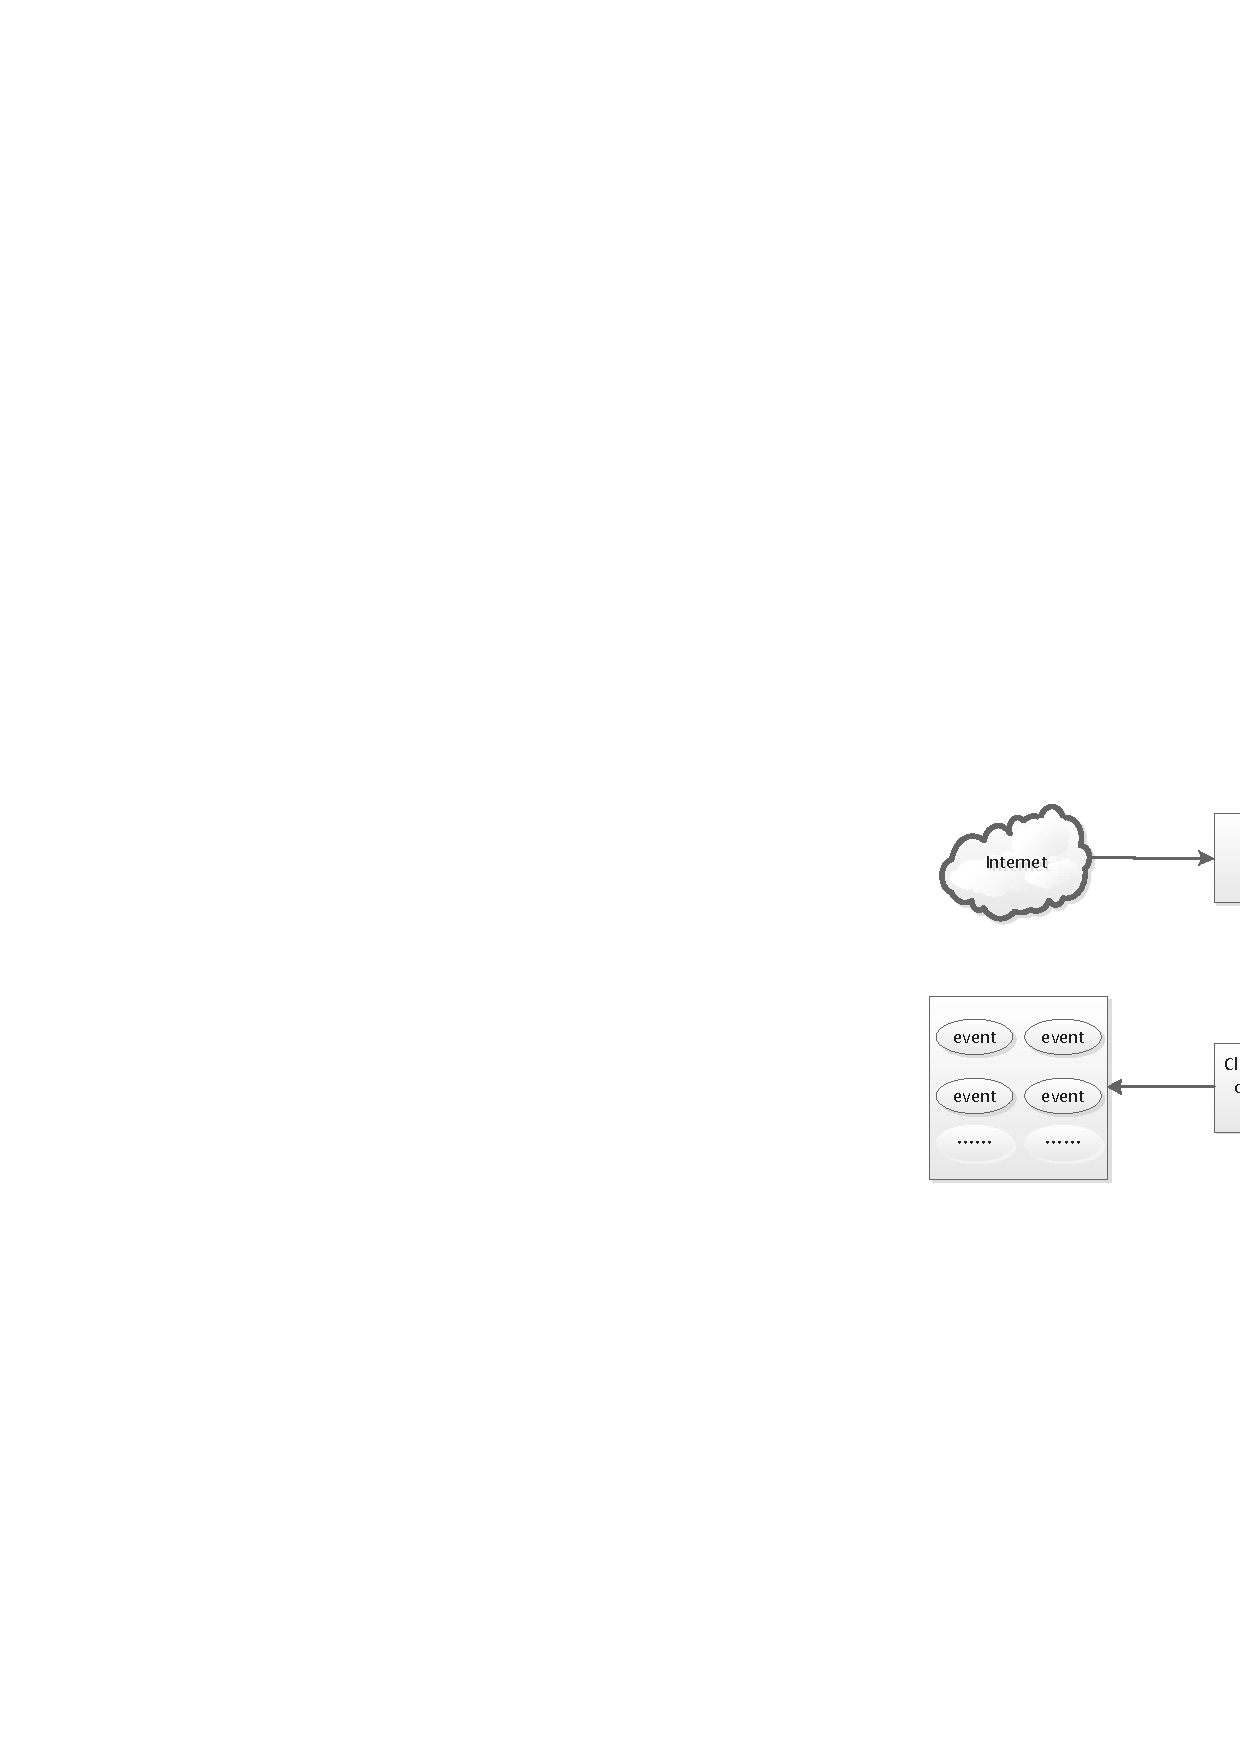
\includegraphics[width=2.5in]{process}
\caption{The process of this society news detection system}
\label{systemprocess}
\end{figure}

\subsection{Topic web crawler on society news}

Topic web crawler constitutes the news acquistion module. It's the data source of this system and determines whether the contents of the entire wealth of information systems as well as timely news updates. The principle of a web crawler is descriped in  Fig \ref{fig:crawler}. Firstly, crawler will get the souce code of web pages based on the initial URL seeds.Secondly,  after parsing the URL from these pages, the crawler will remove all the URLs that already crawled and put new coming URLs into the queue. Thirdly, the crawler will do this loop untils the queue is empty or some specific stop condition reached. 
\begin{figure}
\centering
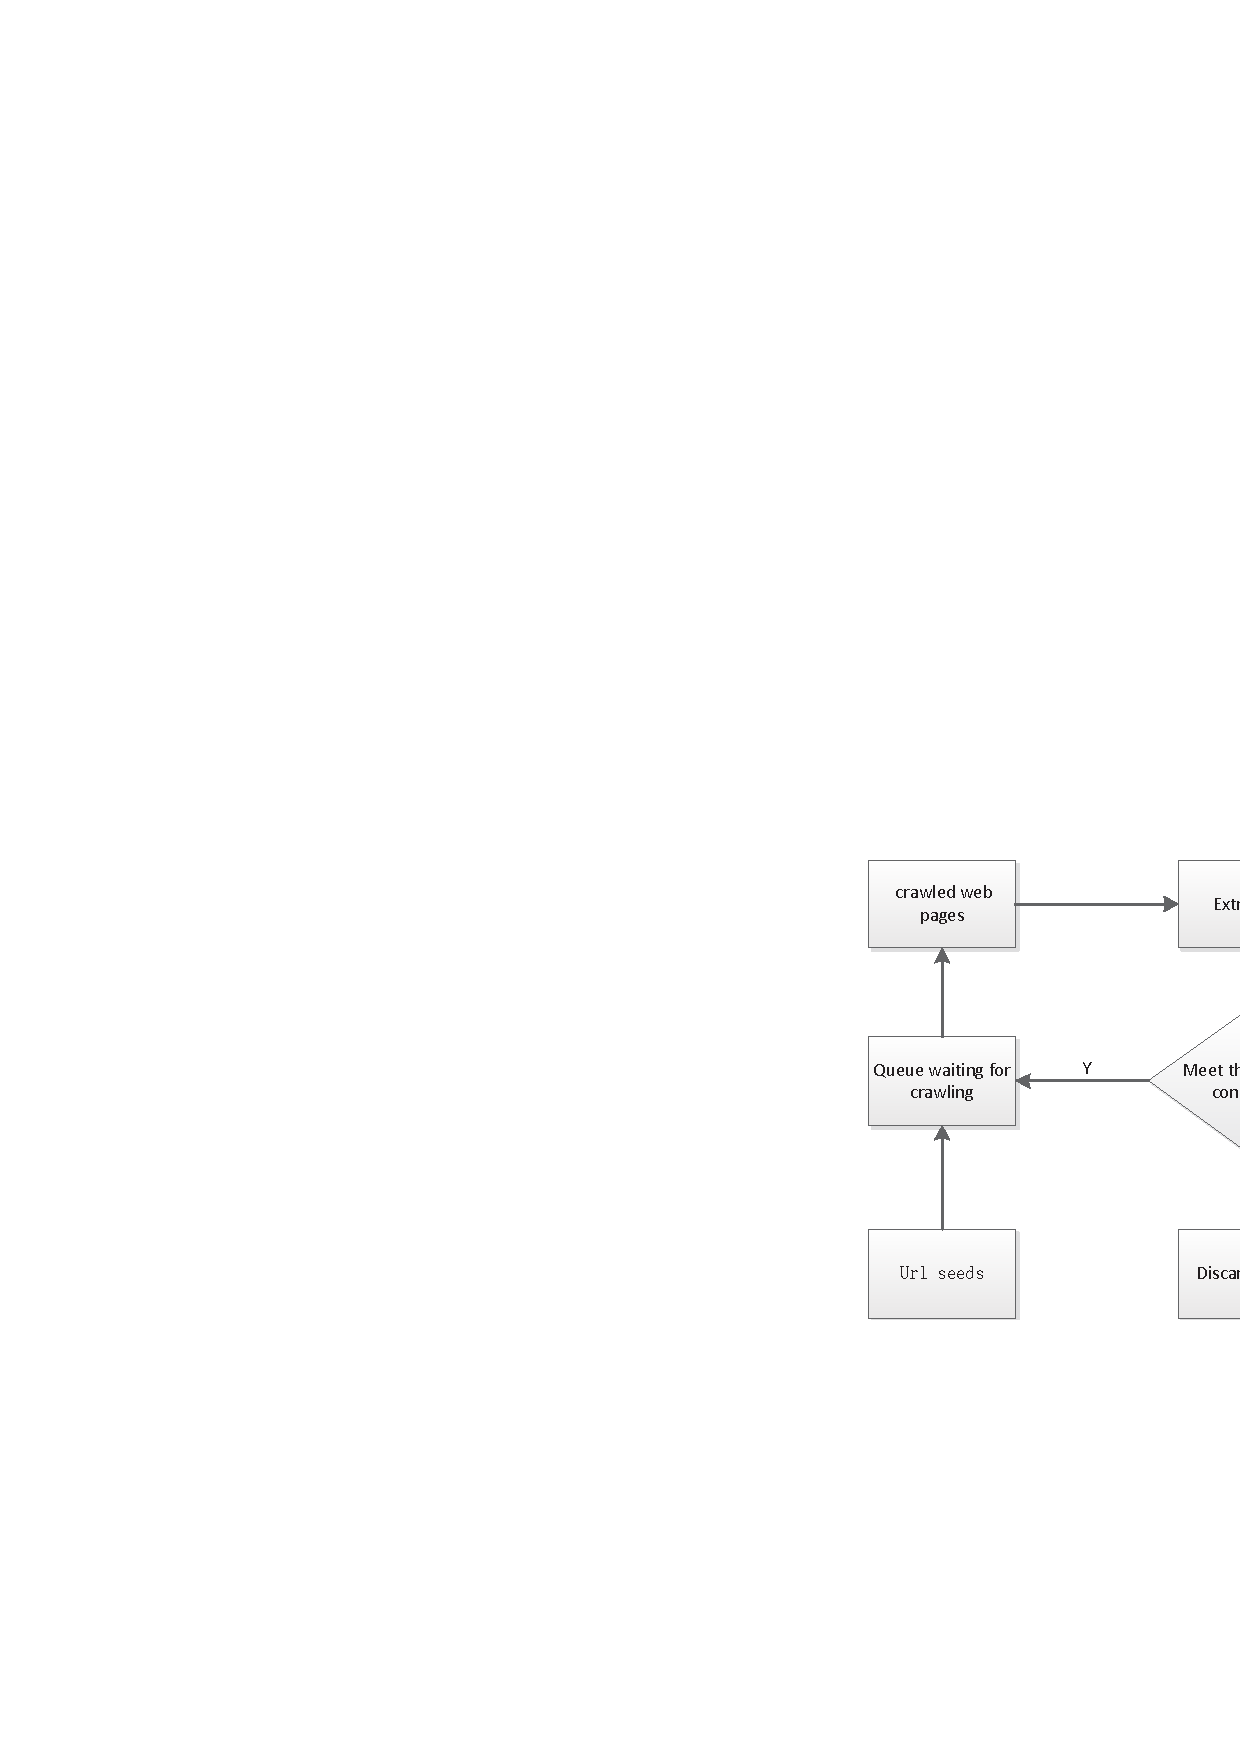
\includegraphics[height=2.5in]{crawler}
\caption{the principle of web crawler}
\label{fig:crawler}
\end{figure}
The goal of society news topic web crawler is to do classification to the pages , store the news belong to society news and remove others. We get the train data from some big news media website, crawl pages from different channels and labeled them as their channel. For example, we label the news from sports channel to sport class. With this kind of training data, we train a classificator based on native bayes algorithm.Firstly, we cut the sentence into words with word parser and  remove stop words and . Secondly ,  we count the occurrence number of each word group by labels. Thirdly, we can compute  whether the new comming pages belong to the society news group by fomular \ref{nativebayes}
\begin{equation}
P(C_i|X) = \frac{P(X|C_i) P(C_i)}{P(X)}
\end{equation}
\begin{equation}
P(X|C_i) = \prod_{k=1}^n P(X_k|C_i) = P(x_1|C_i) * P(x_2|C_i)* \dots * P(x_n|C_i)
\end{equation}


\subsection{Web content parsing}

As the web pages crawled by web crawler contain much irrelevant information, like html tags, javascript and so on, we need preprocess the data before using it, which consists of two steps: content extraction and inverse index establishment.

A combination of a segmentation-like approach and a density-based approach  are used to extract the main content  of web page[7]. Firstly, we construct a DOM tree for the original web pages. And then convert the DOM tree to more easily processed BLE\&IE blocks. BLE are defined that elements displayed as block margins in a new line with independent height and width. They can only contain text or IE.A BLE\&IE block is a labeled ordered tree that is converted from a node tree by some specific operations. The root of a BLE\&IE block is a BLE. A regular expression , $(IE|text)*p?q*|l*|t*$, used to match the blocker from the source code .

After converting the DOM to BLE\&IE blocks, we process them with a density-based content extract algorithm to distinct the content from noisy data. The density of a node or a BLE\&IE block is the ratio of TextLength to TagLength. And the ratio is based on such a fact that in HTML documents, contents always contain large numbers of characters and need comparatively fewer characters to describe their tags, while texts in noises always contain small numbers of characters and need comparatively more characters to describe their tags. And only the nodes with higher densities than threshold can be regarded as candidate content. The procedure of the above description can be expressed as follows:
\begin{algorithm}
\end{algorithm}

\subsection{Society events detection}
According to the definition of event, a series of news stories having a same or similar topic can be called an event. 
The goal of society events detection is that cluster the big volumn society news into different events.  The detection of event divide in two steps: news representation and event detection.

\subsubsection{News representation and similiarty matric}

We express each news text with a vector, and each element in vector presents the weight of term t in document d. Here we compute the weight with TFIDF, which is showed as below:
\begin{equation}
w(t,d) = \frac{d_t}{|d|} * log(\frac{N+0.5}{N_t=1})
\end{equation}
Where $d_t$ means the frequency of term $t$ in document $d$, $| d|$ is the number of terms document $d$ contains, $N_t$ is the number of documents that contain term $t$, $N$ is the number of documents in the corpus.
Then we compute the similarity of two documents using the expression below:
\begin{equation}
Sim(d_i, d_j) =  \frac{\sum_{t \in (d_i \bigcap d_j)}w(t,d_i)*w(t,d_j)}{\sqrt{\sum_{t \in d_j} w(t,d_i)^2 } * \sqrt{\sum_{t \in d_j} w(t,d_j)^2}}
\end{equation}

\subsubsection{event detection}
With the expression above, we can obtain the similarity between any two documents and generate the similarity matrix. Then we can utilize the undirected graph to discover news reports with the same topic and cluster them together. In the undirected graph, each node presents a document. If there is an edge between two nodes, we say that the two documents have some relationship and the weight of the edge presents the similarity of the two documents. Here we defined a threshold parameter $\theta$, and connect two nodes with the weighted edge only when the similarity value is larger than the threshold. Finally, nodes at a same undirected graph consist of a news event, which can be showed as follows:

\subsection{Event summarization}
Our system also provides a functional module of automatic abstract for news event after the event discovery step so that users can get the useful information about the event more quickly. In our system, we extract sentences with a centroid-based method. Firstly, we use latent semantic analysis (LSA), a mathematical technique, to derive latent semantics from news. Secondly, we compute the distance between each sentence and the cluster centroid. Thirdly, the weight of each sentence can be obtained with a linear combination of the distance and the position where the sentence is located. Finally, we select the salient sentences with top weight and the minimum redundancy.

\subsubsection{Sematic analysis}

Here we use latent semantic analysis (LSA), a mathematical technique, to derive latent semantics from news. The process starts with the construction of a word-by-sentence matrix $A$, where each row indicates a word, each column indicates a sentence, and $a_{ij}$ indicates the weight of word $w_i$ in sentence $s_j$. Since every word does not normally appear in each sentence, the matrix $A$ is usually sparse. We then apply the singular value decomposition (SVD) to the matrix $A$, which is defined as:
\begin{equation}
A = U \Sigma V^T
\end{equation}
Where $U$ is an $m×n$ matrix whose columns are called left singular vectors, $\Sigma$ is an $n×n$ diagonal matrix whose diagonal elements are non-negative singular values sorted in descending order, and $V$ is an $n×n$ matrix whose columns are called right singular vectors.

Next, we perform a dimension reduction to the diagonal matrix $\Sigma$ by cutting down some elements in it and we get matrix $\Sigma '$. Then a new matrix $A'$ is reconstructed by multiplying three matrices as follows:
\begin{equation}
A'=U'\Sigma'V'^T \approx A
\end{equation}
Where $\Sigma$' represents the semantic space that can derive latent semantic structures from $A$, $U'$ and $V'$ is the dimension reduced matrices correspond to $U$ and $V$ respectively. Each column of $A'$ denotes the semantic sentence representation, and each row denotes the semantic word representation.

\subsubsection{Distance from the centroid}
A centroid is a set of words that are statistically important to a cluster of documents, which represents the core idea of an event. The closer with centroid, the more important information does the sentence contain. Here we use cosine similarity to express the distance between sentence and centroid. And the larger similarity value means the more important sentence.

Firstly, we generate the centroid of the cluster using the top K weighted words and phrases, which can be expressed as $S_c=(w_1,w_2,…,w_k)$. Then, we can calculate the similarities between each sentence and centroid and sort sentences by the similarity value descendingly.
\begin{equation}
W_D(S_i)  = Sim(S_i, S_c) =\frac{ \overrightarrow{S_i} \cdot \overrightarrow{S_c}  }{|S_i||S_c|}
\end{equation}
where $ \overrightarrow{S_i}$ is the vector of sentence $S_i$ and $\overrightarrow{S_c}$ is the vector of centroid $S_c$.

\subsubsection{Sentence Position}
Generally, sentences located at the head position contain more useful information than those at the tail position, so we should assign higher weight to former sentences. Here we simply compute the positional value of sentence by inverse the sentence position in document.
\begin{equation}
W_p(S_i) = \frac{1}{i}
\end{equation}

\subsubsection{Sentence Selection}
After the former steps, we can obtain sentence weight by linearly combining the centroid value and the positional value, which can be defined as follows:
\begin{equation}
W(S_i) = \lambda W_D(S_i) + (1- \lambda) W_p(S_i)
\end{equation}
Then the top N weighted sentences are selected as the candidate abstract sentences. 

\subsection{Experiments}

\subsubsection{Topic Web Crawler}


\subsubsection{Event detection}



\subsection{Conclusion}


\subsection{Subsection Heading Here}
Subsection text here.


\subsubsection{Subsubsection Heading Here}
Subsubsection text here.


% An example of a floating figure using the graphicx package.
% Note that \label must occur AFTER (or within) \caption.
% For figures, \caption should occur after the \includegraphics.
% Note that IEEEtran v1.7 and later has special internal code that
% is designed to preserve the operation of \label within \caption
% even when the captionsoff option is in effect. However, because
% of issues like this, it may be the safest practice to put all your
% \label just after \caption rather than within \caption{}.
%
% Reminder: the "draftcls" or "draftclsnofoot", not "draft", class
% option should be used if it is desired that the figures are to be
% displayed while in draft mode.
%
%\begin{figure}[!t]
%\centering
%\includegraphics[width=2.5in]{myfigure}
% where an .eps filename suffix will be assumed under latex, 
% and a .pdf suffix will be assumed for pdflatex; or what has been declared
% via \DeclareGraphicsExtensions.
%\caption{Simulation Results}
%\label{fig_sim}
%\end{figure}

% Note that IEEE typically puts floats only at the top, even when this
% results in a large percentage of a column being occupied by floats.


% An example of a double column floating figure using two subfigures.
% (The subfig.sty package must be loaded for this to work.)
% The subfigure \label commands are set within each subfloat command, the
% \label for the overall figure must come after \caption.
% \hfil must be used as a separator to get equal spacing.
% The subfigure.sty package works much the same way, except \subfigure is
% used instead of \subfloat.
%
%\begin{figure*}[!t]
%\centerline{\subfloat[Case I]\includegraphics[width=2.5in]{subfigcase1}%
%\label{fig_first_case}}
%\hfil
%\subfloat[Case II]{\includegraphics[width=2.5in]{subfigcase2}%
%\label{fig_second_case}}}
%\caption{Simulation results}
%\label{fig_sim}
%\end{figure*}
%
% Note that often IEEE papers with subfigures do not employ subfigure
% captions (using the optional argument to \subfloat), but instead will
% reference/describe all of them (a), (b), etc., within the main caption.


% An example of a floating table. Note that, for IEEE style tables, the 
% \caption command should come BEFORE the table. Table text will default to
% \footnotesize as IEEE normally uses this smaller font for tables.
% The \label must come after \caption as always.
%
%\begin{table}[!t]
%% increase table row spacing, adjust to taste
%\renewcommand{\arraystretch}{1.3}
% if using array.sty, it might be a good idea to tweak the value of
% \extrarowheight as needed to properly center the text within the cells
%\caption{An Example of a Table}
%\label{table_example}
%\centering
%% Some packages, such as MDW tools, offer better commands for making tables
%% than the plain LaTeX2e tabular which is used here.
%\begin{tabular}{|c||c|}
%\hline
%One & Two\\
%\hline
%Three & Four\\
%\hline
%\end{tabular}
%\end{table}


% Note that IEEE does not put floats in the very first column - or typically
% anywhere on the first page for that matter. Also, in-text middle ("here")
% positioning is not used. Most IEEE journals/conferences use top floats
% exclusively. Note that, LaTeX2e, unlike IEEE journals/conferences, places
% footnotes above bottom floats. This can be corrected via the \fnbelowfloat
% command of the stfloats package.




% conference papers do not normally have an appendix


% use section* for acknowledgement
\section*{Acknowledgment}


The authors would like to thank...


% trigger a \newpage just before the given reference
% number - used to balance the columns on the last page
% adjust value as needed - may need to be readjusted if
% the document is modified later
%\IEEEtriggeratref{8}
% The "triggered" command can be changed if desired:
%\IEEEtriggercmd{\enlargethispage{-5in}}

% references section

% can use a bibliography generated by BibTeX as a .bbl file
% BibTeX documentation can be easily obtained at:
% http://www.ctan.org/tex-archive/biblio/bibtex/contrib/doc/
% The IEEEtran BibTeX style support page is at:
% http://www.michaelshell.org/tex/ieeetran/bibtex/
%\bibliographystyle{IEEEtran}
% argument is your BibTeX string definitions and bibliography database(s)
%\bibliography{IEEEabrv,../bib/paper}
%
% <OR> manually copy in the resultant .bbl file
% set second argument of \begin to the number of references
% (used to reserve space for the reference number labels box)
\begin{thebibliography}{1}

\bibitem{IEEEhowto:kopka}
H.~Kopka and P.~W. Daly, \emph{A Guide to \LaTeX}, 3rd~ed.\hskip 1em plus
  0.5em minus 0.4em\relax Harlow, England: Addison-Wesley, 1999.

\end{thebibliography}

\bibliographystyle{IEEEtran}
\bibliography{IEEEabrv,../../bib/news}


% that's all folks
\end{document}


